\lstdefinelanguage{XML} {
  morestring=[s][\color{mauve}]{"}{"},
  %morestring=[s][\color{black}]{>}{<},
  morecomment=[s]{<?}{?>},
  morecomment=[s][\color{dkgreen}]{<!--}{-->},
  stringstyle=\color{black},
  identifierstyle=\color{lightblue},
  keywordstyle=\color{red},
  morekeywords={fires}% list your attributes here
}

\chapter{QES-Fire}

\section{Introduction}

QES-Fire \cite{Moody2022,Moody2023} is a dynamically coupled wildfire progression model based in the QES framework. QES-Fire uses the solver from QES-Winds to couple atmospheric winds with fire-induced winds to create a 3-D wind field. The wind field then drives a 1-D rate of spread (ROS) model that advances the perimeter at all points along the fire front using the level set method. A graphical representation of the fire model is shown in Fig. \ref{fig:fire_flow}.   

\begin{figure}[H]
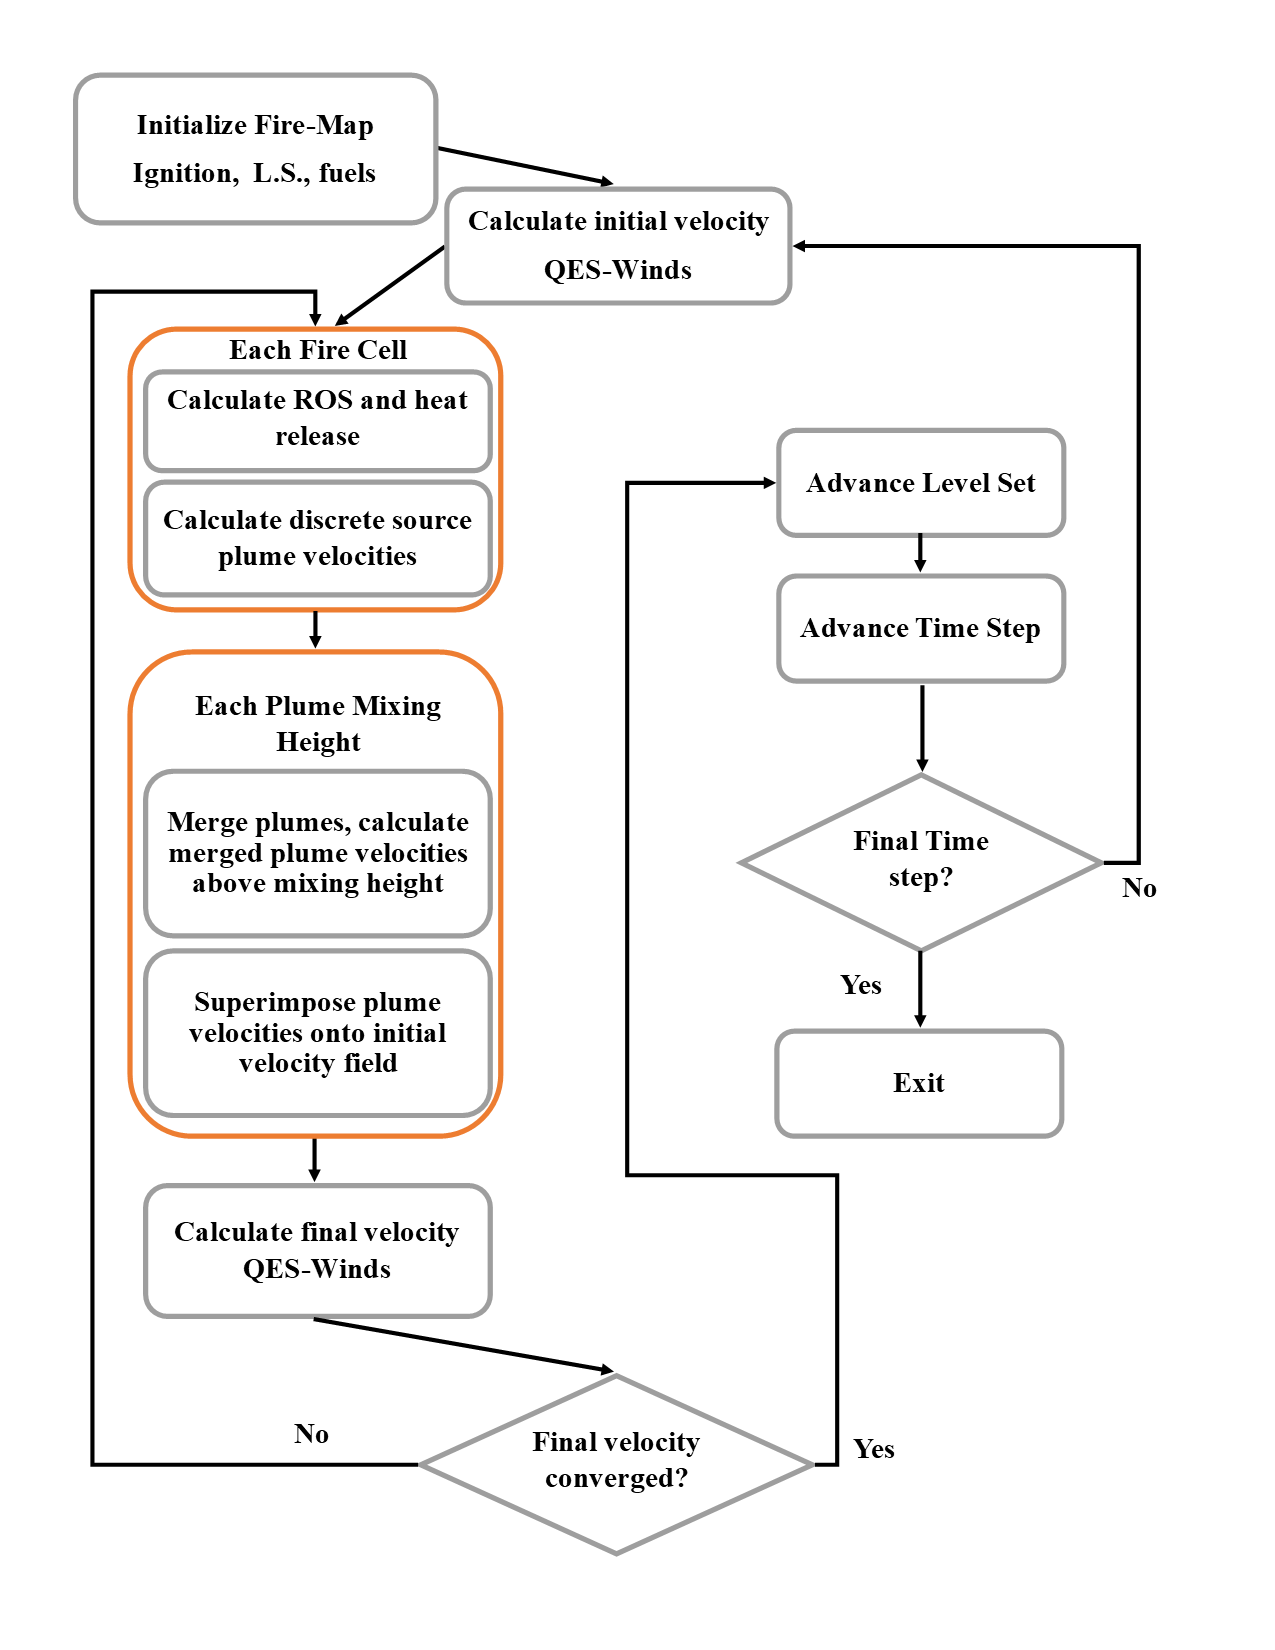
\includegraphics[width=9cm]{Images/Fire-Flowchart.png}
\caption{Flowchart for QES-Fire}
\label{fig:fire_flow}
\end{figure}

\subsection{Fire-Induced Winds}

QES-Fire couples the atmospheric and fire-induced winds using a unique multiscale approach. Wind parameterization is based on the Baum and McCaffrey \cite{Baum1989} buoyant plume rise model and the Kaye and Lindon \cite{kaye_linden_2004} turbulent axisymmetric plume merging model. QES-Fire calculates nondimensional parameterized winds for distinct plumes, and then scales the nondimensional winds by the heat release to get a full 3-D wind field. Since the parameterization for each plume is linear, distinct plumes can be vectorially added using superpostion. QES-Winds treats each individual cell as a distinct plume at the surface. As these buoyant plumes rise, QES-Fire uses the methodology of Kaye and Lindon to merge the plumes together. The merging height is calculated for nearby plumes, and the Baum and McCaffrey parameterization is applied and superimposed with all other wind vectors, from the surface to the merging height for each plume. From the initial merging height, QES-Fire then calculates a new merge height for plumes that have not yet merged. The process continues until all plumes have merged, or the domain height is reached, whichever occurs first. 

The fire-induced winds are then sumperimposed on the initial background atmospheric winds calculated by QES-Winds. The QES-Winds solver is then run again to solve the difference from the initial to the final velocity using the variational method described in QES-Winds. 

\subsection{Rate of Spread}

QES-Fire uses two ROS models to drive the fire progression. The first is the most widely used in the US, the Rothermel ROS model \cite{Rothermel1972}. The Rothermel model is an empirical model that uses parameters for 13 fuel classes developed by Anderson \cite{anderson1982} and later expanded to 40 fuel classes by Scott and Burgan \cite{scott2005standard}. Other inputs for the Rothermel model include wind at mid-flame height, slope of the terrain, and fuel moisture. 

The second ROS model is the simplified physics Balbi model \cite{Balbi2020}. The Balbi model uses simplifications for flame geometry, radiative and convective heat transfer, and flame angle to iteratively solve for ROS. Other inputs to the Balbi model include fuel parameters, wind at the mid-flame height, terrain slope, and fuel moisture. Since the Balbi model is an iterative model and requires an initial guess for ROS, QES-Fire uses the Rothermel model to initialize the Balbi model. 

The output of the ROS model includes the 1-D ROS normal to the fire front at a given point along the perimeter of the fire, the height of the flame, the depth of the flame, and the time for the cell to burnout. An additional output of the ROS model is the heat release per grid cell, used by QES-Fire to scale the parameterized fire-induced winds. 

\subsection{Level Set}

The fire front in QES-Fire is tracked and advanced using the level set method \cite{sethian1999}. At initialization all burning cells are set as the zero level of the level set, $\phi_{i,j}(t=0) = 0$, where $\phi$ is the level set function, and the subscripts $i$ and $j$ are the cell indices in the $x$ and $y$ directions respectively. As the fire front cannot burn over ground where it has already passed, an upwind numerical scheme to advance the level set is appropriate, and is calculated as 

\begin{equation}\label{eq:levelSet}
    \phi_{i,j} = \phi_{i,j}^{0} - \Delta t\left[max(F_{i,j},0)\nabla^{+} + min(F_{i,j},0)\nabla^{-}\right],
\end{equation}

where the superscript $0$ is the previous value for the level set function, $\Delta t$ is the timestep, $F_{i,j}$ is the forcing per cell, $\nabla^{+}$ is the forward in space gradient of $\phi$, and $\nabla^{-}$ is the backwards in space gradient of $\phi$. $F_{i,j}$ is the calculated ROS in a narrow band surrounding the zero level set.

\section{Parameter Files}

The XML parameter file has the following structure, with the XML elements corresponding to a different section of the model. See QES-WINDS for simulation, domain, meteorological, building, vegetation, and file options. Here, the XML structure for fire is presented.

\begin{lstlisting}[language=XML]
<QESWindsParameters>
    <simulationParameters>
        <!-- SEE QES-WINDS -->
    </simulationParameters>

    <metParams>
        <!-- SEE QES-WINDS -->
    </metParams>

    <buildingsParams>
        <!-- SEE QES-WINDS -->
    </buildingsParams>

    <vegetationParams>
        <!-- SEE QES-WINDS -->
    </vegetationParams>

    <turbParams>
        <!-- SEE QES-TURB -->
    </turbParams>

    <fires>
        <!-- FIRE PARAMETERS HERE-->
    </fires>

    <fileOptions>
        <!-- SEE QES-WINDS -->
    </fileOptions>
</QESWindsParameters>
\end{lstlisting}


\section{Fire XML}
\subsection{Basic Parameters}

The time for the fire simulation to run is defined under <fireDur> in seconds after the initial <timeStamp> in the <metParams> section (see QES-Winds). QES-Fire uses a dynamic timestep with a modified Courant number\cite{Ferziger2002}, $C$ calculated as,
\begin{equation}\label{eq:deltf}
    \Delta t_f = C \frac{max(\Delta x, \Delta y)}{max(\mathrm{ROS})},
\end{equation}
where $\Delta t_f$ is the fire timestep, $\Delta x$ and $\Delta y$ are the cell sizes in the $x$ and $y$ directions, and $max(\mathrm{ROS})$ is the domain wide maximum ROS. QES-Fire is numerically stable and the fire front cannot jump cells when $C\leq 1$. 
\begin{lstlisting}[language=XML]
<fires>
    <!-- Fire simulation time -->
    <fireDur> 3600 </fireDur>
    <!-- Timestep Courant number -->
    <courant> 0.9 </courant>
    <!-- ... -->
</fires>
\end{lstlisting}

\subsection{Fuel Parameters}

QES-Fire fuel elements for each grid cell are initialized through the XML. These include the fuel class, the fuel moisture, and the moisture content of live vegetation. The fuel type is a numeric value from Anderson (1-13) or Scott and Burgan (98-215) and is specified throughout the domain. Furthermore, QES-Fire has the ability to read a geoTiff for heterogeneous fuel beds, with the address to the fuel file location defined using <fuelMap>. If a fuel file is specified, QES-Fire will ignore the fuel type specified. Dead fuel moisture is specified under <fmc> as the fraction of water to fuel mass. Finally, for dynamic conversion of live to dead fuel, the moisture content of live fuel is specified under <cure> as the fraction of water to oven dry fuel mass.

\begin{lstlisting}[language=XML]
<fires>
    <!-- Fuel class -->
    <fuelType> 102 </fuelType>
    <!-- Address to fuel file -->
    <fuelMap>../FireFiles/test.tif</fuelMap>
    <!-- Dead fuel moisture content -->
    <fmc> 0.05 </fmc>
    <!-- Live fuel moisture content -->
    <cure> 0.3 </cure>
    <!-- ... -->
</fires>
\end{lstlisting}
\subsubsection{Ignitions}

QES-Fire must have an initial ignition point specified in the XML. Multiple ignitions may be specified, and all ignitions will occur at the start of the simulation corresponding to the first <timeStep> in the <metParams> section of the XML. For ignitions occurring after the initial start, the user must provide a netCDF file with the structure of 't' = time after simulation start (seconds), 'x' = x location in the domain (meters), and 'y' = y location in domain (meters).

\begin{lstlisting}[language=XML]
<fires>
    <!-- Ignition point in domain -->
    <ignition>
        <!-- Height of flame (meters) -->
        <height> 2 </height>
        <!-- Height of flame base above ground (meters) --> 
        <baseHeight> 0 </baseHeight>
        <!-- X location of ignition point in domain (meters) -->
        <xStart> 200.0 </xStart>
        <!-- Y location of ignition point in domain (meters) -->
        <yStart> 15.0 </yStart>
        <!-- X length of initial igntion (meters) -->
        <length> 6.0 </length>
        <!-- Y width of initial ignition (meters) -->
        <width>  6.0 </width>
    </ignition>
    <!-- Address to ignition file -->
    <igTimes>../FireFiles/FFII.nc</igTimes>
    <!-- ... -->
</fires>
\end{lstlisting}

\subsubsection{Example XML}
The full XML used to run the FireFlux II simulation is included.
\begin{lstlisting}[language=XML]
<QESWindsParameters>
    <simulationParameters>
        <halo_x> 5.0 </halo_x>
        <halo_y> 5.0 </halo_y>
        <domain> 80 150 40 </domain>
        <cellSize> 5.0 5.0 .25 </cellSize>
        <verticalStretching> 0 </verticalStretching>
        <totalTimeIncrements> 1 </totalTimeIncrements>
        <maxIterations> 500 </maxIterations>
        <tolerance> 1e-9 </tolerance>
        <meshTypeFlag> 1 </meshTypeFlag>
    </simulationParameters>
    <metParams>
        <z0_domain_flag> 0 </z0_domain_flag>
        <sensor>
            <site_coord_flag> 1 </site_coord_flag>
            <site_xcoord> 1.0  </site_xcoord>
            <site_ycoord> 1.0 </site_ycoord>
            <timeSeries>
                <timeStamp>2013-01-30T15:04:08</timeStamp>
                <boundaryLayerFlag> 1 </boundaryLayerFlag>
                <siteZ0> 0.1 </siteZ0>
                <reciprocal> 0.0 </reciprocal>
                <height>10.0 </height>
                <speed> 8.9 </speed>
                <direction> 295.0 </direction>
            </timeSeries>
        </sensor>
    </metParams>
    <fires>
        <fireDur> 1200 </fireDur>
        <fuelType> 103 </fuelType>
        <fmc> 0.065 </fmc>
        <cure> 0.3 </cure>
        <ignition>
            <height> 0.25 </height>
            <baseHeight> 0 </baseHeight>
            <xStart> 65.0 </xStart>
            <yStart> 655.0 </yStart>
            <length> 5.0 </length>
            <width> 5.0 </width>
        </ignition>
        <courant> 0.9 </courant>
        <igTimes>../FireFiles/FFII.nc</igTimes>
    </fires>
    <fileOptions>
        <outputFlag>1</outputFlag>
        <outputFields>all</outputFields>
    </fileOptions>
</QESWindsParameters>
\end{lstlisting}
